\chapter{Theoretical Background}\label{ch:theoretical-background}

This chapter is providing the necessary background for the two main pylons of this work, Deep (Machine) Learning and the
protocols that used for the distributed training of the neural networks.


\section{Machine Learning}\label{sec:machine-learning}

Machine learning (ML) is a subset of Artificial Intelligence (AI) algorithms that gives systems the ability to learn in
an automatic way and improve from experience without
being explicitly programmed.
Machine Learning concentrates on the development of computer programs that can reach data and learn from them.
The learning process works with observations or data, such as examples, direct experience, or instruction, to explore
patterns in data and get better decisions based on the
samples we provide.
The primary purpose is to enable the computers to learn without human intervention or assistance
and modify actions accordingly.

\subsection{Learning Paradigms}\label{subsec:learning-paradigms}

The three major learning paradigms are supervised learning, unsupervised learning and reinforcement learning.
They each correspond to a particular learning task.
Below, I will try to introduce them.

{\large \textbf{Supervised Learning}}

Supervised learning algorithms construct a model of data that have both the
inputs and the correct outputs.
The training data and comprises a set of examples.
Each training example has at least one input and the correct output.
Supervised learning algorithms construct an optimized function that predicts the output correlated with new inputs.
The percentage of the prediction accuracy determines how successful the model is.

The types of ML problems that fits in this type of learning are the regression and the classification.
Classification algorithms are used when the outputs are  a set of values, and in regression are a range of arithmetical values.
For example, a classification algorithm that separates tumors, would have an image of a
medical instrument as input, and the type of the tumor as output, namely benign or malignant.

{\large \textbf{Unsupervised Learning}}

In contrast to supervised learning, unsupervised learning algorithms need a collection of data that carries only inputs and aims to discover any pattern in the data, such as groups or clusters of data points.
Consequently, these algorithms use data that have not been labeled to learn from.
Rather than evaluating, unsupervised learning algorithms recognize data patterns and respond
based on the presence or absence of such similarities in each fresh bunch of data.
Unsupervised learning algorithms are mainly applied in Statistics for density estimation.
Yet unsupervised learning encircles more domains such as data feature summary and explain.

In cluster analysis a set of observations is divided into batches subgroups named clusters.
Thus, according to one or more predefined criteria, observations within the same cluster are similar,
while observations extracted from other clusters are divergent.
Various clustering methods generate various assumptions on the structure of the data.
The similarity between members of the corresponding cluster define the success of the method.
Other methods are based on calculated density and graph connectivity.

{\large \textbf{Reinforcement learning}}

Reinforcement learning (RL) is a field of machine learning concerned with how software agents should perform
actions in an environment to maximize some concept of aggregate reward.
RL differs from supervised learning in not needing labeled input/output pairs to be defined,
and in not needing sub-optimal actions to be explicitly corrected.
Instead, the focus is on balancing between exploration (of an unknown area) and exploitation (of current knowledge).
As a result of its abstraction, reinforcement learning is used in many AI fields.
In ML, the environment is modeled as a Markov Decision Process (MDP).
Dynamic programming techniques are used in many RL algorithms.
RL algorithms do not presume the information of a specific algebraic model of the MDP and are used when exact models are infeasible.
RL is a good stuff for Robotics, Bidding and Advertising and building bots for games.

\subsection{Deep Learning}\label{subsec:deep-learning}

Deep learning (DL) is a specific subfield of machine learning.
The 'deep' part in deep learning is not a reference to any kind of deeper understanding achieved by the approach.
Rather, it stands for this idea of consecutive layers of representations.
The number of layers that contribute to a model of the data is called the depth of the model.
Modern deep learning often involves tens or even hundreds of successive layers of representations and they
have all learned automatically from exposure to training data.
Meanwhile, other approaches to machine learning tend to concentrate on learning only one or two layers of
representations of the data.

In DL, the representations of these layered are trained on models called neural networks.
The fundamental part of these networks is the neurons (see figure 2.1).
These are stacked in layers.
The phrase neural network is a reference to neurobiology, but even though basic thoughts in deep learning were
developed influenced by the brain's neural system, DL models differ.
For our purposes, deep learning is a mathematical framework for learning representations from data.

\begin{figure}[H]
    \centering
    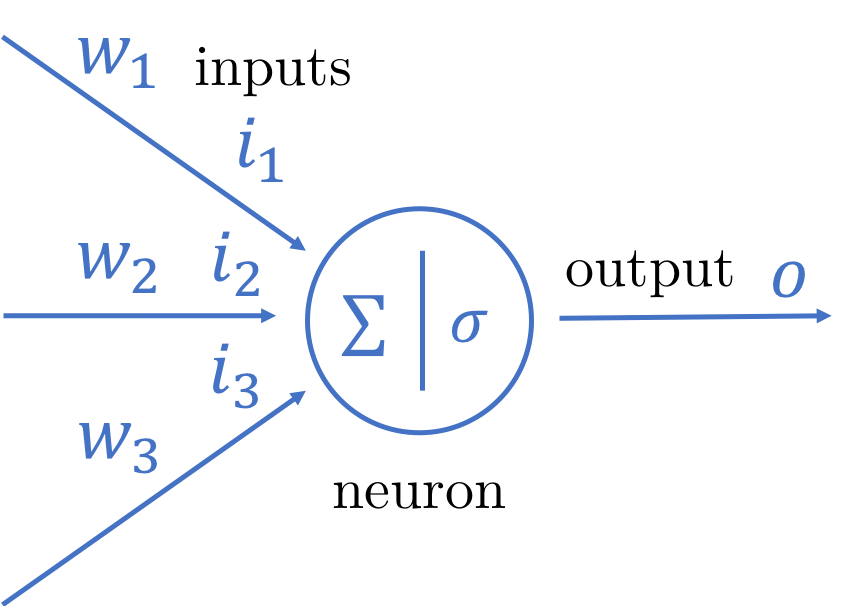
\includegraphics[scale=.40]{./images/background/neuron.png}
    \caption{An artificial neuron}
    \label{fig:neuron_fig}
\end{figure}

The simplest architecture of an Artificial Neural Network (ANN) is shown in Figure 2.2.
This architecture is known as Feed forward Neural Network (FFNN) and is the most basic and widely used artificial neural network.
Consider dealing with an image classification problem.
The input of the network, consists of the distinct dataset sample.
For this instance, this is an image pixels.
It propagates the values over the hidden layers via the edges which are weighted until the last layer is reached.
This is the output layer.
The output represents the odds of the sample to belong to each one of the different classes, for example,
the probabilities that the input image represents a benign tumor or a malignant one.
At every neuron, a non-linear function can be triggered.
Although this type of neural network has been successfully tested in many tasks, the
temporal condition that it describes sequential data is not taken into account.
Each sample has the fate to be distinct.

\begin{figure}[H]
    \centering
    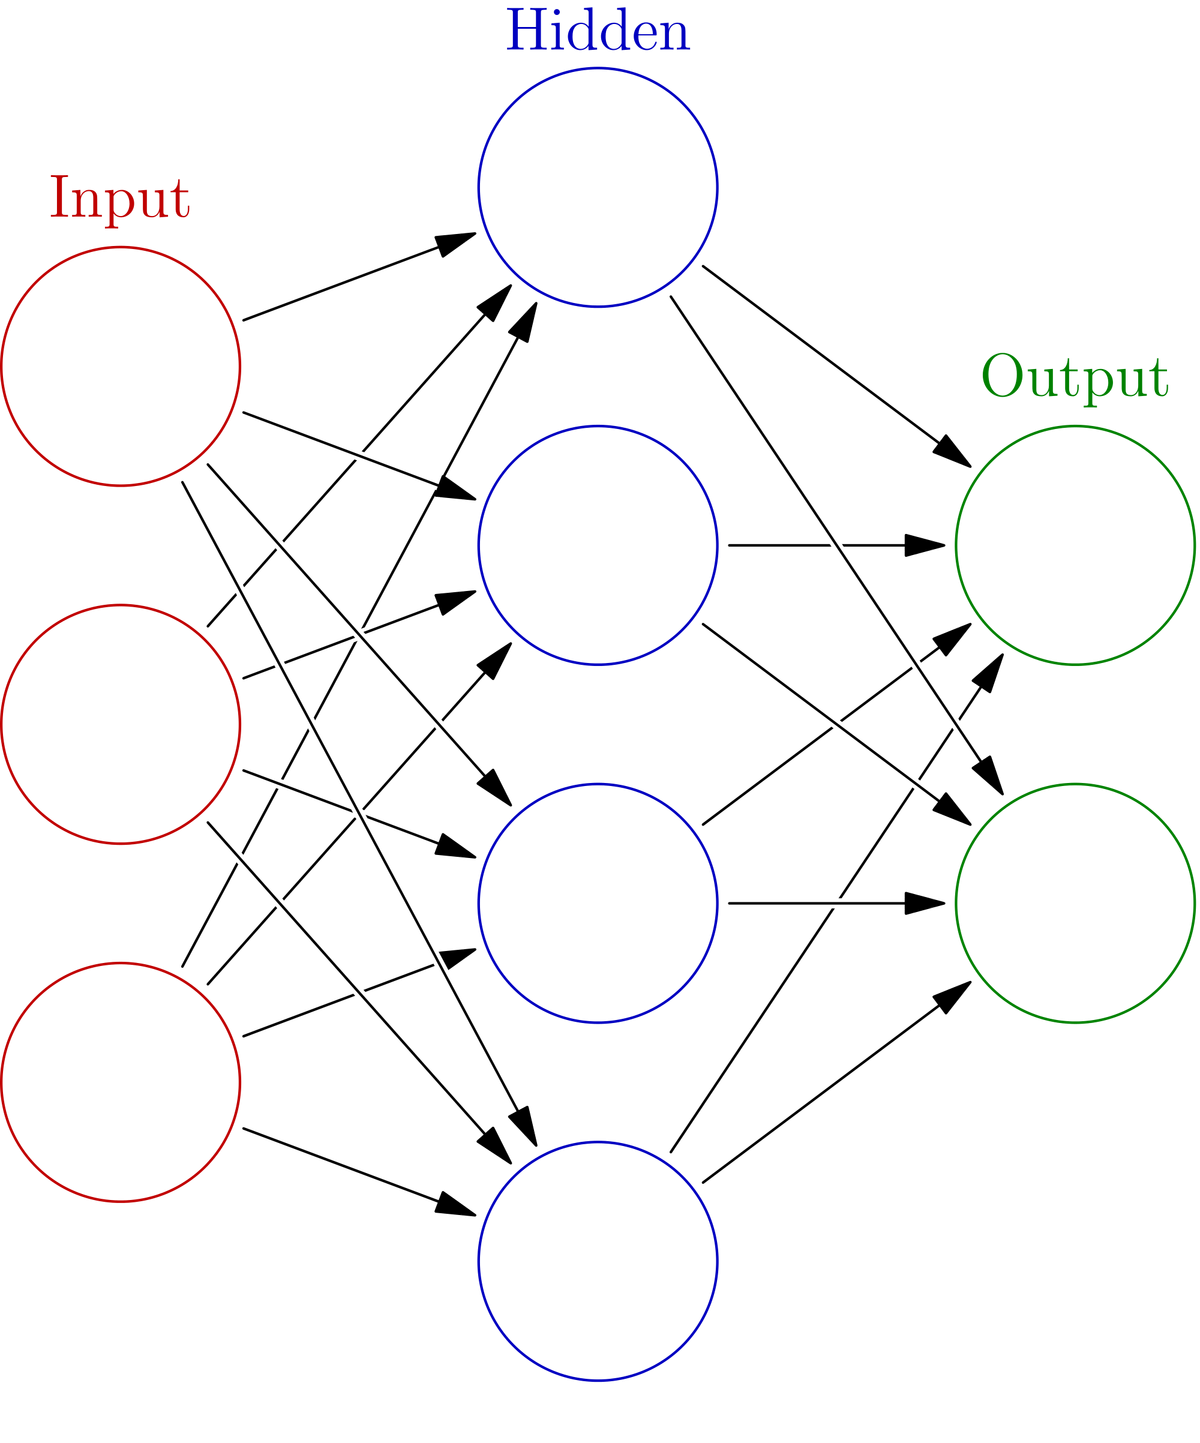
\includegraphics[scale=.20]{./images/background/simplefnn.png}
    \caption{A Feedforward Neural Network with only one hidden layer}
    \label{fig:ffnn_fig}
\end{figure}

The specification of what a layer does to its input data is stored in the layer’s weights,
which in essence are a collection of numbers.
In technical terms, we would assume that the transformation implemented by a layer is parameterized by its weights.
Weights are also sometimes called the parameters of a layer.
If we want to achieve a successful learning process, we must find a set of values for the weights of all
layers in a network and this will correctly
map example inputs to their correlated targets.

\begin{figure}[H]
    \centering
    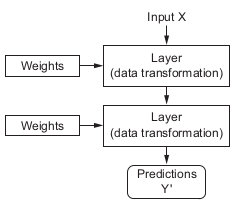
\includegraphics[scale=1.]{./images/background/params.png}
    \caption{A neural network is parameterized by its weights}
    \label{fig:params}
\end{figure}

To succeed in learning, we need to be able to measure how far this output is from what you expected.
This is the job of the loss function of the network.
The loss function grabs the predictions of the network and the actual target which is the desired
output and computes a distance score,
capturing how well the network has done on this specific example.

\begin{figure}[H]
    \centering
    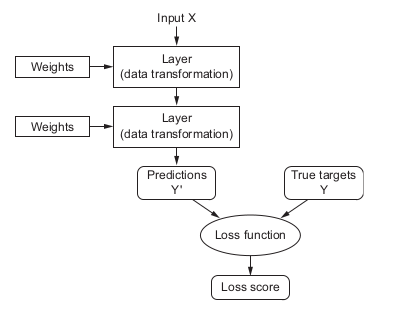
\includegraphics[scale=1.]{./images/background/loss.png}
    \caption{A loss function measures the quality of the network’s output}
    \label{fig:loss}
\end{figure}

The most elemental function is the Mean Squared Error (MSE).
The formula is

\begin{equation}
    MSE(y,\hat{y}) = \frac{1}{n} \sum_{i=1}^{n} (y_i - \hat{y_i})^2 ,\label{eq:equation2}
\end{equation}

where $y$ stands for the target output and $\hat{y}$ is the output that we got from the network.

{\large \textbf{Training Process}}

At first, the weights of the network are initialized with random values, so the network merely
performs a set of random transformations.
Normally, its output is far away from what it should ideally be, and the accuracy is respectively very low.
As the network processes the rest of the examples, it adjusts the weights a little in the correct
direction, and the accuracy increases.
This is the training loop, which, in a sufficient number of iterations, produces weight values that
minimize the loss function.
This process is called Backpropagation (BP).
Actually, this is the backward propagation of the error.

Backpropagation is an algorithm that computes the chain rule, with a precise order of operations that is highly useful.
Let x be a real number, and let f and g both be functions mapping from a real number to a real number.
Assume that y = g(x) and z = f(g(x)) = f(y).
Then the chain rule asserts that

\begin{equation}
    \frac{dz}{dx} = \frac{dz}{dy} \frac{dy}{dx}\label{eq:equation3}
\end{equation}

We can generalize this regarding a scalar case.
Assume that $x \in \mathbb{R}^m , y \in \mathbb{R}^n , g $ maps from $\mathbb{R}^m$ to $\mathbb{R}^n$ , and $f$ maps
from $\mathbb{R}^n$ to $\mathbb{R}$.
If $y = g(x)$ and $z = f(y)$, then

\begin{equation}
    \frac{\partial z}{\partial x_i} = _{j}^{} \frac{\partial z}{\partial y_j} \frac{\partial y_j}{\partial x_i}\label{eq:equation4}
\end{equation}

If I write with vectors, then we get

\begin{equation}
    \nabla_x z = \frac{\partial y}{\partial x}^\top \nabla_y z\label{eq:equation5}
\end{equation}

where $\frac{\partial y}{\partial x}$ is the $n \times m$ Jacobian matrix of $g$ .

From this we understand that the gradient of a variable $x$ can be reached by multiplying a Jacobian matrix
$\frac{\partial y}{\partial x}$ by a gradient $\nabla_y z$.
The backpropagation algorithm comprises performing such a Jacobian-gradient product for each operation in the graph.
Let us see BP in more detail with two algorithms.

\textbf{Forward pass}

Below I have a forward pass through a standard Deep Neural Network (DNN) and the calculation of the cost function.
The loss $L(\hat{y}, y)$ depends on the output $\hat{y}$ and on the target $y$.
For integrity, this approach uses only a single input example x.
Practical applications should work with mini-batches.

\begin{algorithm}[H]
    \caption{Forward pass in a standard DNN}
    \begin{algorithmic}
        \REQUIRE net depth $l$
        \REQUIRE $W^{(i)} , i \in {1, \cdots , l}$ , the weights
        \REQUIRE $b^{(i)} , i \in {1, \cdots , l}$ , the biases
        \REQUIRE input $x$
        \REQUIRE target output $y$
        \STATE $h^{(0)} = x$
        \FOR{$k \gets 1$ to $l$}
        \STATE $a^{(k)} = b^{(k)} + W^{(k)} h^{(k-1)}$
        \STATE $h^{(k)} = f(a^{(k)})$
        \ENDFOR
        \STATE $\hat{y} = h^{(l)}$
        \STATE $J = L(\hat{y},y)$
    \end{algorithmic}\label{alg:nn_forward_pass}
\end{algorithm}

\textbf{Backward pass}

Momentarily, I introduce the backward pass for the DNN of Algorithm~\ref{alg:nn_forward_pass}.
This computation produces the gradients on the activations $a^{(k)}$ for each layer $k$, starting from the output layer and moving backward to the first hidden layer.
From these gradients, which can be described as evidence of how each layer’s output should adjust to reduce error, one can get the gradient on the parameters of each layer.
Generally, the main purpose is to minimize these gradients, following several iterations.
This process is also called as Gradient Descent (GD).

\begin{algorithm}[H]
    \caption{Backward pass in a standard DNN}
    \begin{algorithmic}
        \STATE $g \leftarrow \nabla_{\hat{y}} J = \nabla_{\hat{y}} L(\hat{y},y)$
        \FOR{$k \gets l$ to $1$}
        \STATE $g \leftarrow \nabla_{a^{(k)}} J = g \odot f'(a^{(k)})$
        \STATE $\nabla_{b^{(k)}} J = g + \lambda \nabla_{b^{(k)}}$
        \STATE $\nabla_{W^{(k)}} J = g h^{(k-1)\top} + \lambda \nabla_{W^{(k)}}$
        \STATE $g \leftarrow \nabla_{h^{(k-1)}} J = W^{(k)\top} g$
        \ENDFOR
    \end{algorithmic}\label{alg:nn_backward_pass}
\end{algorithm}

A network with the smallest loss is one for which the outputs are as close as they can be to the targets.
This is a trained network.

There are many different architectures of neural networks each with their unique strengths.
For instance, Convolutional Neural Networks (CNN) show very effective results in image and video recognition.
In this work, I will focus on Recurrent Neural Networks.

\subsection{Recurrent Neural Networks}\label{subsec:recurrent-neural-networksrnn}

A Recurrent Neural Network (RNN) is one powerful model from the deep learning family that has
shown incredible results in the last years.
It proposes to produce predictions on sequential data by utilizing a powerful memory-based architecture.
But how is it differs from a feed-forward neural network?
An FFNN works as a mapping function, where a single input is associated with a single output.
In this type, no two inputs share knowledge and each moves in
only one direction beginning from the input nodes, accessing
hidden nodes and closing at the output nodes.

\begin{figure}[H]
    \centering
    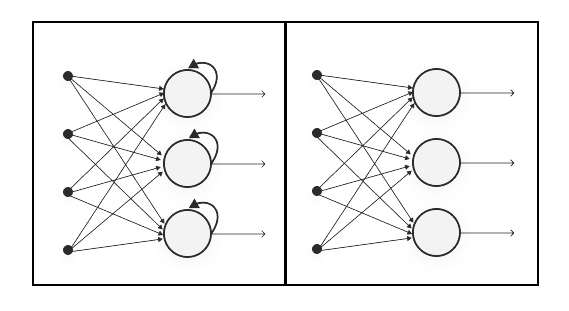
\includegraphics[scale=0.6]{./images/background/rnn.png}
    \caption{At left, this is a Recurrent Neural Network, and at right a Feedforward one.}
    \label{fig:rnn}
\end{figure}

Since a CNN is functional for dealing with a grid of values $X$ such as a photo,
a RNN is a network that is specially designed for dealing with a sequence of
values $x^{(1)} , \ldots , x^{(\tau)}$.

To jump from a FFNN to a RNN, we need to consider the idea of splitting parameters through other parts of a model.
Such splitting is especially significant when an exact chunk of information can happen at various positions within the sequence.
For instance, look at  the two sentences “I visited Italy in 2019” and “In 2019, I visited Italy.”
If we request a ML model to read each words and obtain the year in which the reciter visited Italy, we would like it to see
the year 2019 as the important piece of information, either it appears in the sixth word or the second word of the sentence.
Assume that we have trained an FFNN that processes sentences of fixed length.
A conventional fully connected FFNN would have separate parameters for each input feature, so it would need to learn
all of the rules of the language separately at each position in the sentence.
By comparison, an RNN shares the same parameters across a lot of time steps.


{\large \textbf{Basic Structure}}

Now, I will introduce the forward pass equations of an RNN represented in Figure~\ref{fig:rnn_unfolded}.
The figure does not define either the type of activation function for the hidden units or the loss function.
Suppose we have the hyperbolic tangent (tanh) activation function and the MSE as the loss function.
Additionally, we suppose that the output is distinct as if the RNN is used to forecast characters or words.

A straightforward manner to describe discrete variables is to rate the output $\textbf{o}$ as providing the probabilities of each possible value.
Now, it can be applied the softmax function to get a vector $\hat{y}$ across the output.
Forward pass starts with a definition of the initial state $h^{(0)}$.
Next, for each time step from $t=1$ to $t=\tau$, we use the latter equations for updating:

\begin{equation}
    a^{(t)} = b + W \cdot h^{(t-1)} + U \cdot x^{(t)}\label{eq:equation6}
\end{equation}
\begin{equation}
    h^{(t)} = tanh(a^{(t)})\label{eq:equation7}
\end{equation}
\begin{equation}
    o^{(t)} = c + V \cdot h^{(t)}\label{eq:equation9}
\end{equation}
\begin{equation}
    \hat{y}^{(t)} = softmax(o^{(t)})\label{eq:equation8}
\end{equation}

where $\textbf{b}$ and $\textbf{c}$ are the biases along with the weight matrices $\textbf{U}$,
$\textbf{V}$, and $\textbf{W}$, for input-to-hidden, hidden-to-output, and hidden-to-hidden connections, respectively.
This is an example of a RNN that connects an input sequence to an output one.
Both sequences have the same length.
The entire loss for a given sequence matched with a sequence of output values would
then be the summation of the losses over all the steps.

Calculating the loss function gradient concerning the weights has a lot of cost.
The gradient calculation requires making a forward pass moving left to right, tailgated by a backward pass.
The runtime is $O(\tau)$ cannot be cut by parallel execution because the forward pass graph is essentially
sequential since each time step needs to be calculated after the previous one.
The backpropagation algorithm utilized to the unfolded graph is called backpropagation through time (BPTT).

\begin{figure}[H]
    \centering
    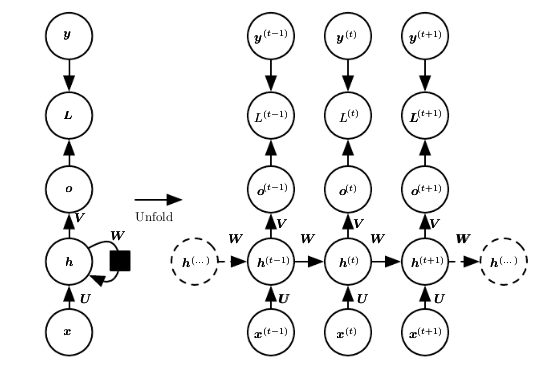
\includegraphics[scale=0.8]{./images/background/rnn_unfolded.png}
    \caption{Unfolding an RNN}
    \label{fig:rnn_unfolded}
\end{figure}

In Figure~\ref{fig:rnn_unfolded}, at left we have the RNN and its loss have described with recurrent connections.
At right, it is the same scene as a time-unrolled graph,
where each node is now correlated with a specific time step.


{\large \textbf{Training and Evaluation}}

Calculating the gradient through a recurrent neural network is straightforward.
One simply applies the generalized backpropagation Algorithm~\ref{alg:nn_backward_pass} to the unfolded graph.

To obtain some feeling for how the BPTT acts, we present an example of how to compute gradients by BPTT for the RNN equation 2.4 above.
The nodes of our graph combine the weights $U, V, W, b$, and $c$ as well as the sequence of nodes indexed by $t$ for $x^{(t)}, h^{(t)}, o^{(t)}$, and $L^{(t)}$.
For each node $N$, we ought to calculate the gradient $\nabla_N L$ recursively, based on the gradient calculated at nodes that follow it in the graph.
We begin the recursion with the nodes directly preceding the terminal loss

\begin{equation}
    \frac{\partial L}{\partial L^{(t)}} = 1\label{eq:equation10}
\end{equation}

In this derivation, we suppose that the outputs $o^{(t)}$ are managed as the argument to the softmax function to get the vector $\hat{y}$ of probabilities over the output.
Besides, we suppose that the loss is the negative log-likelihood of the true target $y^{(t)}$.
The gradient $\nabla_{o^{(t)}} L$ on the outputs at time step $t$, for all $i, t$, is as arises:

\begin{equation}
    (\nabla_{o^{(t)}} L)_i = \frac{\partial L}{\partial o^{(t)}_i} = \frac{\partial L}{\partial L^{(t)}} \frac{\partial L^{(t)}}{\partial o^{(t)}_i} = \hat{y}^{(t)}_i - 1_{i,y^{(t)}}\label{eq:equation11}
\end{equation}

We work our way from the opposite direction, beginning from the tail of the sequence.
At the last time step $\tau, h^{(\tau)}$ just has $o^{(\tau)}$ as a descendent.
Therefore, we calculate its gradient as,

\begin{equation}
    \nabla_{h^{(t)}} L = V^\top \nabla_{o^{(t)}} L\label{eq:equation12}
\end{equation}

Now we are able to loop back in time to backpropagate gradients through time, from $t = \tau - 1$ down to $t = 1$,
regarding that $h^{(t)}$ (for $t < \tau$) has as descendants both $o^{(t)}$ and $h^{(t+1)}$.
Consequently, its gradient is provided by,

\begin{equation}
    \nabla_{h^{(t)}} L = (\frac{\partial h^{(t+1)}}{\partial h^{(t)}})^\top (\nabla_{h^{(t+1)}} L) (\frac{\partial o^{(t)}}{\partial h^{(t)}})^\top (\nabla_{o^{(t)}} L) \Rightarrow\label{eq:equation13}
\end{equation}
\begin{equation}
    \nabla_{h^{(t)}} L = W^\top (\nabla_{h^{(t+1)}} L) diag(1-(h^{(t+1)})^2) + V^\top (\nabla_{o^{(t)}} L)\label{eq:equation14}
\end{equation}

where $diag(1-(h^{(t+1)})^2)$ registers to the diagonal matrix containing the elements.

Once the gradients on the inner nodes of the graph are collected, we can get the gradients on the parameter nodes.
Due to the weights are shared through many steps, we should get some concern when expressing calculus processes including these variables.
The types we hope to complete working with the backpropagation method of the previous subsection,
which calculates the addition of a single edge in the graph to the gradient.
Nevertheless, the $\nabla_W f$ operator applied in calculus considers the contribution of $W$ to the value of $f$ because of the all edges in the graph.
To fix this doubt, we import fool variables $W^{(t)}$ that are set to be clones of $W$ but with each $W^{(t)}$ used hardly at time step $t$.
Using these symbols, the gradient on the parameters that left is provided by:

\begin{equation}
    \nabla_c L = \sum_t (\frac{\partial o^{(t)}}{\partial c})^\top \nabla_{o^{(t)}} L = \sum_t \nabla_{o^{(t)}} L\label{eq:equation15}
\end{equation}
\begin{equation}
    \nabla_b L = \sum_t (\frac{\partial h^{(t)}}{\partial b^{(t)}})^\top \nabla_{h^{(t)}} L = \sum_t diag(1-(h^{(t)}))^2 \nabla_{h^{(t)}} L\label{eq:equation16}
\end{equation}
\begin{equation}
    \nabla_V L = \sum_t \sum_i (\frac{\partial L}{\partial o^{(t)}_i}) \nabla_V o^{(t)}_i = \sum_t (\nabla_{o^{(t)}} L) h^{(t)^\top}\label{eq:equation17}
\end{equation}
\begin{equation}
    \nabla_W L = \sum_t \sum_i (\frac{\partial L}{\partial h^{(t)}_i}) \nabla_{W^{(t)}} h^{(t)}_i \Rightarrow\label{eq:equation18}
\end{equation}
\begin{equation}
    \nabla_W L = \sum_t diag(1-(h^{(t)}))^2 (\nabla_{h^{(t)}} L) h^{(t-1)^\top}\label{eq:equation19}
\end{equation}
\begin{equation}
    \nabla_U L = \sum_t \sum_i (\frac{\partial L}{\partial h^{(t)}_i}) \nabla_{U^{(t)}} h^{(t)}_i \Rightarrow\label{eq:equation20}
\end{equation}
\begin{equation}
    \nabla_U L = \sum_t diag(1-(h^{(t)}))^2 (\nabla_{h^{(t)}} L) x^{(t-1)^\top}\label{eq:equation21}
\end{equation}

{\large \textbf{Possible issues and Optimization}}

These architectures regularly face long-term dependencies.
The primary problem is that gradients propagated over many stages and conduce to either vanish or explode resulting in much contamination to the optimization.
Even if we suppose that the weights make a reliable network,
the difficulty with long-term dependencies appears from the hugely smaller parameters given to long-term interactions associated with short-term ones.

This problem is particular to RNN. Figure multiplying a weight w by itself a lot of times.
The product $w^t$ will either vanish or explode depending on the magnitude of $w$.
The vanishing and exploding gradient problem for RNNs were separately discovered by many researchers.
Unluckily, to save memories in a way that is robust to small perturbations, the RNN must get in an area of weight range where gradients vanish.
It does not mean that it is difficult to train, but that it may cost much time to learn long-term dependencies
because the signal about these dependencies will tend to be hidden by the smallest changes resulting from short-term dependencies.

{\large \textbf{Long Short Term Memory Networks}}

Long Short Term Memory (LSTM) networks are a special set of RNN, capable of learning long-term dependencies.
They introduced by Hochreiter and Schmidhuber in 1997.
They operate remarkably well on a wide variety of problems.
LSTM networks are explicitly created to bypass the long-term dependency obstacle.
Memorizing information for long periods is reasonably their default behavior.
All recurrent neural networks have the form of a chain of recurring modules of neural networks.
In a traditional RNN, this repeating module will have a very simple composition, such as a single tanh layer.

\begin{figure}[H]
    \centering
    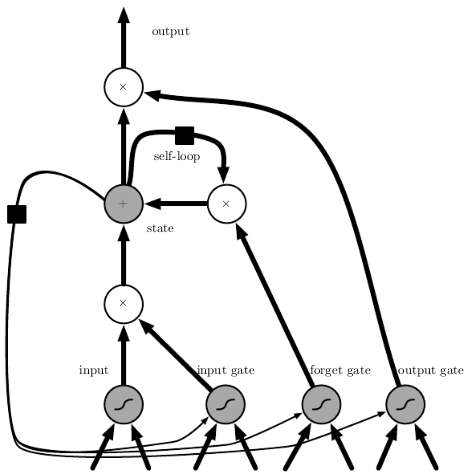
\includegraphics[scale=0.8]{./images/background/lstm.png}
    \caption{The structure of an LSTM cell}
    \label{fig:lstm}
\end{figure}

The smart idea of entering self-loops to build paths where the gradient can remain for long durations is the core of the initial LSTM model.
By securing the parameters of this self-loop gated (controlled by another hidden unit), the time scale of integration can be adjusted dynamically.
The LSTM has been observed notably successful in many applications, such as unconstrained handwriting recognition, speech recognition, and
handwriting generation.

The LSTM block diagram is demonstrated in figure 2.7.
The corresponding forward pass equations are given below.
Instead of a unit that only applies an element-wise nonlinearity to the affine transformation of inputs and recurrent units, LSTM networks have cells that have an internal self-loop,
except that the outer recurrence of the RNN\@.
Each cell has the same inputs and outputs as a common RNN\@.
However, it has more parameters and a system of gating units that control the flow of information.
The most significant part is the state unit $s^{(t)}_i$ that has a linear self-loop.
This self-loop weight is controlled by a forget gate unit $f^{(t)}_i$ (for time step $t$ and cell $i$ ), that defines this parameter between 0 and 1 using a sigmoid function:

\begin{equation}
    f^{(t)}_i = \sigma (b^f_i + \sum_j U^f_{i,j} x^{(t)}_j + \sum_j W^f_{i,j} h^{(t-1)}_j) ,\label{eq:equation22}
\end{equation}

where $x^{(t)}$ is the current input vector and $h^{(t)}$ is the current hidden layer vector,
including the outputs of all the LSTM cells, and $b^f ,U^f , W^f$ are respectively
biases, input weights and recurrent weights for the forget gates.
Consequently, the LSTM cell internal state is updated as follows, but with a conditional self-loop weight $f^{(t)}_i$,

\begin{equation}
    s^{(t)}_i = f^{(t)}_i s^{(t-1)}_i + g^{(t)}_i \sigma (b_i + \sum_j U_{i,j} x^{(t)}_j + \sum_j W_{i,j} h^{(t-1)}_j) ,\label{eq:equation23}
\end{equation}

where $b, U$ and $W$ respectively declare the biases, input weights and recurrent weights into the LSTM cell.
The \textbf{external input gate} unit $g^{(t)}_i$ is calculated similarly to the forget gate, but with its own parameters,

\begin{equation}
    g^{(t)}_i = \sigma (b^g_i + \sum_j U^g_{i,j} x^{(t)}_j + \sum_j W^g_{i,j} h^{(t-1)}_j) ,\label{eq:equation24}
\end{equation}

The output $h^{(t)}_i$ of the LSTM cell can also be shut off by the output gate $q^{(t)}_i$, which also uses a sigmoid unit for gating,

\begin{equation}
    h^{(t)}_i = tanh(s^{(t)}_i) q^{(t)}_i\label{eq:equation25}
\end{equation}
\begin{equation}
    q^{(t)}_i = \sigma (b^o_i + \sum_j U^o_{i,j} x^{(t)}_j + \sum_j W^o_{i,j} h^{(t-1)}_j) ,\label{eq:equation26}
\end{equation}

which has parameters $b^o, U^o, W^o$ for its biases, input weights and recurrent.

LSTM networks have been proved to learn long-term dependencies more easily than conventional RNN\@.
At first, they tested on artificial data sets designed for examining the ability to learn long-term dependencies.
After that, this time had tested on challenging sequence processing tasks where state-of-the-art performance was achieved.


\section{Geometric Monitoring Methods}\label{sec:geometric-monitoring-methods}

Monitoring complex and continuous queries on distributed streams are by default a complicating problem.
Sharfman, Schuster, and Keren in~\cite{sharfman_geometric_2007}~\cite{sharfman_aggregate_2007}, initially presented the Geometric Monitoring (GM) method for monitoring non-linear functions.
This method is a communication protocol that resolves this problem efficiently by using convex analysis theory.
Vasilis Samoladas and Minos Garofalakis in~\cite{garofalakis_sketch-based_2013}~\cite{garofalakis_distributed_nodate}~\cite{samoladas_functional_nodate}, generalized and improved this method with the Functional Geometric Monitoring (FGM) method by decreasing dramatically the network cost communication.
In this section, we will introduce the theoretical background of these two geometric monitoring methods.

In this point, it is very important to define some stuff.
The following algorithms fit in star network topologies.
Thus, there are two fundamental entities, the local nodes/sites and the hub/coordinator.
Consider we have $k$ nodes/sites.

\subsection{Geometric Monitoring}\label{subsec:geometric-monitoring}

    At each site, a local data stream is received and stands for a high dimensional vector $V$ $\in$ $\mathbb{R}^D$.
Let define $S_i(t)$, $i$ $\in$ $[0,k]$ the local state vector.
Assume w.l.o.g that in a random time step $t$, the coordinator holds the true global stream and
this is the average vector $S(t)$ of local state vectors of all sites.
So,

\begin{equation}
    S(t) = \frac{1}{k} \sum_{i=1}^{k} S_i(t)\label{eq:equation}
\end{equation}

Consistently, a continuous query on the global state $Q(S(t))$ is a complicated non-linear function of $S$.
To decrease communication costs among the hub and the local sites, the user can permit a small bounded error $\epsilon$ to the query answer.
Specifically, the coordinator does not hold the actual global stream state $S(t)$, but a enough close estimation of it, $E(t)$,
providing an approximate query response $Q(E(t))$, with a warranty that at any time step $t$ will be

\begin{equation}
    Q(S(t)) \in (1 \pm \epsilon) Q(E(t))\label{eq:equation27}
\end{equation}

In a same way, we define $E_i$ as the last sent vector to the coordinator by the site $i$.
Therefore,

\begin{equation}
    E(t) = \frac{1}{k} \sum_{i=1}^{k} E_i(t)\label{eq:equation28}
\end{equation}

Additionally, until the global estimate E is updated, and as long as the true global stream state $S(t)$ is inside the admissible region

\begin{equation}
    A = \{ x \in V | Q(x) \in (1 \pm \epsilon)Q(E) \} ,\label{eq:equation29}
\end{equation}

there is no need a site to communicate with the hub.
When this condition has been violated, it is necessary to update the estimate $E$ to compromise in the Eq.~\ref{eq:equation27}.

The GM protocol works in rounds.
Every round starts when a new estimate $E$ is aggregated in the coordinator and lasts until it will be updated again.

At the beginning of each round the hub the initial global state vector is equal with

\begin{equation}
    S(t_0) = \frac{1}{k} \sum_{i=1}^{k} E_i = E.\label{eq:equation30}
\end{equation}

The next step for the hub is to adopt and send to sites a 'good' safe zone $Z \subseteq A$ where $Z$ is a convex subset of $A$ and $E \in Z$.

Each node, at any time $t$  maintains a drift vector $X_i(t)$.
All nodes drift vectors compose the current global state.
Thus,

\begin{equation}
    S(t) = \frac{1}{k} \sum_{i=1}^{k} X_i(t)\label{eq:equation31}
\end{equation}

{\large \textbf{Basic structure of protocol}}

At the beginning of each round, when $t = t_0, X_i(t_0) = E$ for all sites $i = 1, \dots, k$.
As a local stream update appears at a site $i$ at time $t$, the invariant is managed by adding to $Xi$ the vector $S_i(t) - S_i(t-1)$.
Therefore, the actual difference of the local stream state $E$ of each site is equal to $X_i(t) - E$.
Obviously, at the kickoff of each round the drift vector is equal to the zero vector for all $i = 1, \dots, k$.

Each local site observes the local condition $X_i(t) \in Z$.
If this condition continues at each site, then by the convexity of $Z$ and the drift invariant, it will be true that $S(t) \in Z$ too, and consequently, $S(t) \in A$.
When a violation of the local condition $X_i \in Z$ happens, the site $i$ wave the hub and the round ends.
The coordinator says to the sites to broadcast the updates that occurred during the round.
This can be arranged by shipping each local state vector Xi to the coordinator.
Then, the coordinator refreshes E and starts a new round.

To be more specific, the tool that helps protocol monitor the local conditions is the variance of the current local stream.
So,

\begin{equation}
    Var[S(t)] = \frac{1}{k} \sum_{i=1}^{k} ||S(t) - E ||^2_2\label{eq:equation32}
\end{equation}

The protocol receives a positive and real user-defined number as threshold $T$.
While the variance of local streams described by the above equation is below the threshold T,
the nodes continue to monitor this condition without communication with the hub.
Differently, there is a need for communication with the hub.
The local violation for a node $i$ is described by the below condition.

\begin{equation}
    ||X_i(t) - E ||^2_2 > T\label{eq:equation33}
\end{equation}

{\large \textbf{Rebalancing the GM protocol}}

When you inspect the basic algorithm of the GM protocol you may mention that when a local violation occurs at a site $i$,
it is not undoubtedly the fact that $S \in Z$.
This might be true, in all other remote sites $j \neq i$, is still the case that $X_j \in Z$.
To be more accurate, consider that after the beginning of a round, all the stream updates have been sent to the remote site $i$,
whose drift vector $X_i$ does not belong in the convex set $Z$ but it’s close enough.
Next, it is true that all the other drift vectors $X_j$ are yet equal to $E$, for $j \neq i$.
Now, it is more obvious to realize that it is probably liberal to end the round at the first local violation.

These methods are principally heuristic and their goal is to reset some of the drift vectors so as to restore the local conditions at all sites with the dream of additional reduction of the communication cost.
Firstly, we define the set $B = \{i\}$, where $i$ is the site that yielded a local violation.
Iteratively, we add each new local site index to $B$, and at each step, we compute the mean state vector $X_B$  for all nodes $\in B$.
If $X_B \in Z$, we reset the drift vector that for all the nodes $\in B$ to $X_B$ and the round resumes regularly.
Else, if $|B| = k$, the round comes to an end.


The goal of the rebalancing methods is to prolong the round life.
There is not any mathematical proof that it is causal, but many experimental researches have confirmed that such heuristic methods can achieve better performance.

\subsection{Functional Geometric Monitoring}\label{subsec:functional-geometric-monitoring}

Let's explore the idea of a safe state in a monitoring algorithm.
The system is in a safe state while $\frac{1}{k} \sum_{i=1}^{k} X_i = S \in A$.
In the meaning of the GM protocol, system safety is only monitored by observing all local conditions $\land_{i=1}^k X_i \in Z$, where $Z$ is a convex subset of the admissible region $A$\@.
When this becomes false, the system restores it, either by starting a new round or by rebalancing.

On the contrary, FGM uses a real function $\phi : \mathbb{R}^D \rightarrow \mathbb{R}$.
Each remote site $i$, for $i = 1, \dots , k$, holds its $\phi$-value, or the value of function $\phi$ on their state vector $X_i$ as it becomes updated.
Thus, system safety is ensured while the global summation of those one-dimensional projections sum $ \psi = \sum_{i=1}^{k} \phi(X_i)$ is non-negative.


{\large \textbf{Mathematical definitions and theorems}}

Underneath, we introduce some significant definitions and theorems that are needed to comprehend the FGM protocol.

\begin{definition}[Safe function]
    A function $\phi : \mathbb{R}^D \rightarrow \mathbb{R}$ is safe for admissible region $A$, if, for all $X_i \in \mathbb{R}^D, i = 1, \dots, k$,
    \begin{center}
        $\sum_{i=1}^{k} \phi(X_i) \geq 0 \Rightarrow \frac{\sum_{i=1}^{k} X_i}{k} \in A$
    \end{center}

\end{definition}

\begin{theorem}
    For any set $A$, if $\phi$ is safe for $A$, then exists a \textbf{concave} function $\zeta \geq \phi$ which is also safe for $A$.
\end{theorem}

Based on the above theorem, the FGM protocol limits its application exclusively to concave safe functions.
For any function $\phi$, define the level set of $\phi$, as

\begin{center}
    $L(\phi) = \{x \in \mathbb{R}^D | \phi(x) \geq 0\}$
\end{center}

For $\phi$ to be safe for some $A$, it is essential that $L(\phi) \subseteq A$.
This is also satisfactory for a concave function $\zeta$.



\begin{prop}
    A concave function $\zeta$ is safe for $A$, if and only if, $L(\zeta) \subseteq A$.
\end{prop}
\begin{proof}
    To prove sufficiency, consider $L(\phi) \subseteq A$.
    By the definition of a concave function, for any $k \geq 1$,
    \begin{center}
        $\zeta\left(\frac{\sum_{i=1}^{k} X_i}{k}\right) \geq \frac{1}{k} \sum_{i=1}^{k} \zeta(X_i)$
    \end{center}
    Next, $\frac{1}{k} \sum_{i=1}^{k} \zeta(X_i) \geq 0$ implies $\zeta(S) \geq 0$, and thus $S \in L(\zeta) \subseteq A$
\end{proof}

Moreover, if $\zeta$ is concave, then the set $Z = L(\zeta)$ is either convex and closed.
Hence, a concave safe function $\zeta$ for an admissible region $A$ can be described as a functional representation for a convex safe zone $L(\zeta) \subseteq A$.
In this way, FGM is conceptually a generalization of GM\@.
Below we define a safe zone function.

\begin{definition}[Safe zone function]
    Given an admissible region $A$ and a reference point $E$, a safe zone function $\zeta$ is a concave function which is safe for $A$, and $\zeta(A) > 0$.
\end{definition}

A 'good' safe zone massively depends on the quality of the safe zone function.
Here in~\cite{garofalakis_distributed_nodate} are described the principles for the quality of a safe zone function
where safe zone functions are used in the compositional design of high-end safe zones for complicated queries.
The problem of defining safe zone functions for specific queries can be beneficial, particularly in ML problems.


{\large \textbf{Basic structure of protocol}}

The FGM protocol also works in rounds.
Monitoring the threshold condition

\begin{equation}
    \sum_{i=1}^{k} \phi(X_i) \leq 0\label{eq:equation34}
\end{equation}

over the duration of the round.
At the beginning of a round, the coordinator has a perfect knowledge of the current state of the system $E = S$.
It selects an $(A, E, k)$-safe function $\phi$, where $A$ is the admissible region, $E$ is the current estimate and $k$ is the number of local nodes.
At any point in time, assume $\psi = \sum_{i=1}^{k} \phi(X_i)$.

The \textbf{round's} steps are:

\begin{enumerate}
    \item At the beginning of a round, the coordinator ships $\phi$ to every site (it is sufficient to ship vector E).
    Local sites initialize their drift vectors to 0.
    With these settings, initially it is $\psi = k \phi(0)$.
    \item Next, the hub defines a number of subrounds, which will be described in detail below.
    At the end of all subrounds, we 'll have $\psi > \epsilon_\psi k \phi(0)$, for some small $\epsilon_\psi$, which usually is set to $0.01$.
    \item At the end, the hub ends the round by collecting all drift vectors and updating $E$.
\end{enumerate}

The goal of each subround is to check the condition $\psi \leq 0$ coarsely, with a precision of $\theta$, achieving this with as little communication as possible.
The \textbf{subround's} steps are:

\begin{enumerate}
    \item At the beginning of a subround, the coordinator knows the value of $\psi$.
    It calculates the subround’s quantum $\theta = -\psi /(2k)$, and sends $\theta$ to each local site.
    In addition, the hub initializes a counter $c = 0$.
    Each local site holds its initial value $z_i = \phi(X_i)$, where $2k\theta = \sum_{i=1}^{k} z_i$.
    Moreover, each local site initializes a counter $c_i = 0$.
    \item Each local site $i$ keeps its local drift vector $X_i$ , as it makes stream updates.
    When $X_i$ is updated, site $i$ updates its counter,
    
    \begin{equation}
        c_i = \max\{c_i, \lfloor\frac{\phi(X_i) - z_i}{\theta}\rfloor\} \label{eq:equation34b}
    \end{equation}

    If this update increases the counter, the local site sends a message to the coordinator, with the increase to $c_i$.
    \item When the coordinator receives a message with a counter increment from a site, it adds the increment to its global counter $c$.
    If the global counter $c$ is bigger than $k$, the hub ends the subround by collecting all $\phi(X_i)$ from all local sites, recomputing $\psi$.
    If $\psi \geq \epsilon_\psi k \phi(0)$, the subrounds end, else another subround begins.
\end{enumerate}
